\begin{frame}{The Multifrontal QR method}
  \begin{overlayarea}{\textwidth}{1cm}
    \only<1>{The original \dr{multifrontal method} by Duff \&
        Reid '83 can be extended to \dr{QR} factorization of sparse
      matrices.

      This method is guided by a graph called \alert{\it elimination
        tree}:}%
    \only<2-3>{The tree is traversed in \db{topological order} (i.e.,
      bottom-up) and, at each node, two operations are performed:}%
    \only<4->{Typically \dr{two sources of parallelism} are exploited
      in the multifrontal method}
  \end{overlayarea}

  \vspace{0.2cm}

  \begin{columns}
    \begin{column}{0.6\textwidth}
      \begin{overlayarea}{\textwidth}{6cm}
        \only<1>{\begin{itemize}
          \item each node is associated with a relatively small
            \alert{dense} matrix called \db{frontal matrix} (or
            \db{front}) containing k pivots to be eliminated along
            with all the other coefficients concerned by their
            elimination.
          \end{itemize}}\only<2-3>{
          \begin{itemize}
          \item<2-3> \alert{assembly}: coefficients from the original
            matrix associated with the pivots and  \alert{\it
              contribution blocks} produced by the treatment of the child
            nodes are \alert{stacked}  to form the frontal matrix.
          \item<3-> \alert{factorization}: the $k$ pivots are eliminated
            through a complete dense QR factorization of the frontal matrix. As a
            result we get:
            \begin{itemize}
            \item part of the global $R$ and $Q$ factors.
            \item a triangular \db{\it contribution block} that will be
              assembled into the father's front.
            \end{itemize}
            
          \end{itemize}}\only<4->{\begin{itemize}
          \item<5-> \dr{tree-level} parallelism: frontal matrices located in
            independent branches in the tree can be processed in
            parallel.
          \item<6-> \dr{node-level} parallelism: large frontal matrices
            factorization may be performed in parallel by multiple
            threads.
          \end{itemize}}
      \end{overlayarea}
    \end{column}
    \begin{column}{0.4\textwidth}
      \begin{center}
        \only<1>{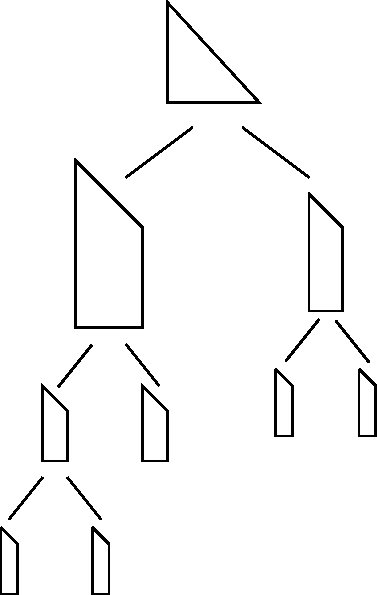
\includegraphics[width=\textwidth]{figures/etree}}%
        \only<2>{\includegraphics[width=\textwidth]{figures/etree2}}%
        \only<3->{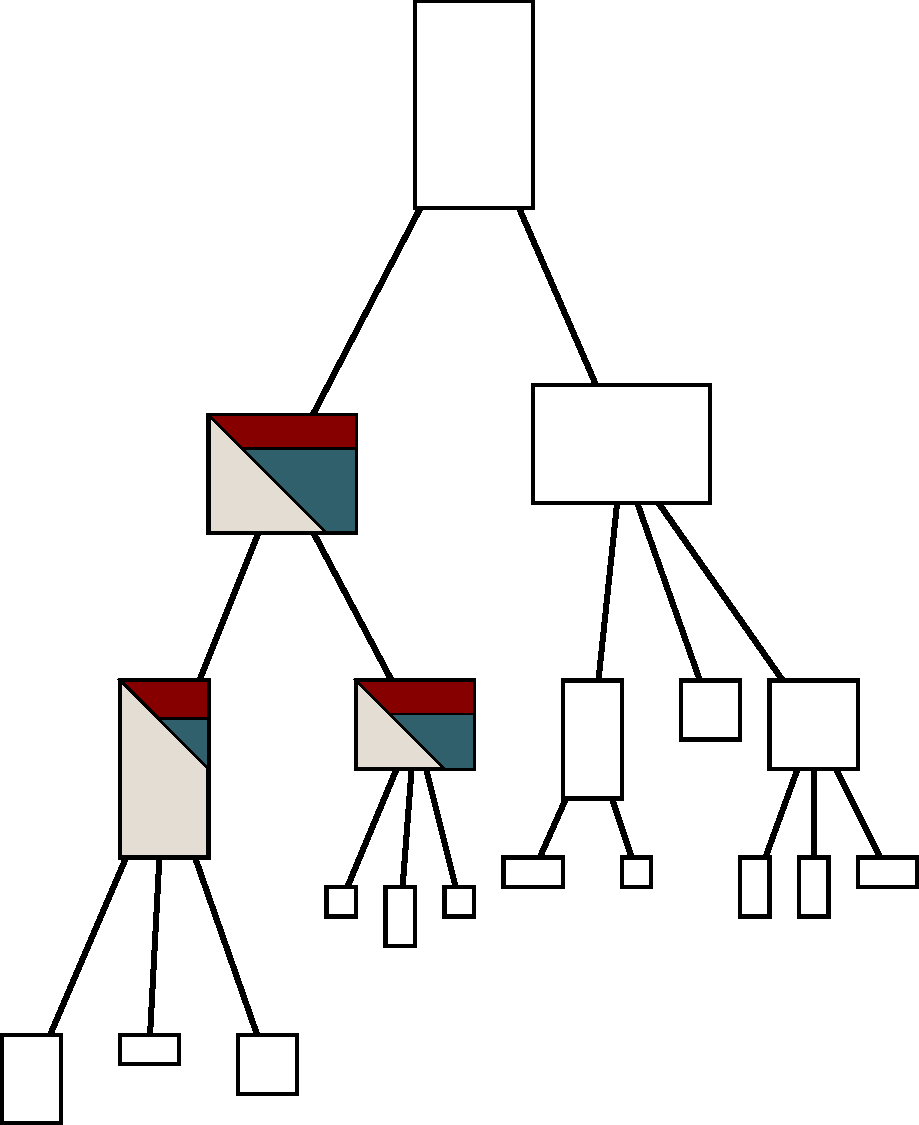
\includegraphics[width=\textwidth]{figures/etree3}}%
      \end{center}
    \end{column}
  \end{columns}
\end{frame}

\begin{frame}[fragile,t]{The task-based multifrontal QR factorization}
  \dr{Sequential} multifrontal $QR$ code

  \begin{columns}[t]
    \begin{column}{0.45\textwidth}
      \begin{center}
        \includegraphics[width=0.6\textwidth]{figures/tree}
      \end{center}
    \end{column}
    \begin{column}{0.55\textwidth}
      \lstinputlisting{listings/mf-seq.f90}
    \end{column}
  \end{columns}
\end{frame}

\begin{frame}[fragile,t]{The task-based multifrontal QR factorization}
  \dr{Sequential} multifrontal $QR$ code with 1D block partitioning

  \begin{columns}[t]
    \begin{column}{0.45\textwidth}
      \begin{center}
        \includegraphics[width=0.6\textwidth]{figures/tree_part}
      \end{center}
    \end{column}
    \begin{column}{0.55\textwidth}
      \lstinputlisting{listings/mf-seq-multicore.f90}
    \end{column}
  \end{columns}
\end{frame}

\begin{frame}[fragile,t]{The task-based multifrontal QR factorization}
The tree is transformed into a DAG

\begin{columns}[t]
  \begin{column}{0.45\textwidth}
    \begin{center}
      \includegraphics[width=0.6\textwidth]{figures/tree_part}
    \end{center}
  \end{column}
  \begin{column}{0.55\textwidth}
    \begin{center}
      \includegraphics[width=0.8\textwidth]{figures/tree_dag}
    \end{center}
  \end{column}
\end{columns}

\vspace{0.5cm}

\begin{itemize}
\item Seamless exploitation of tree and node parallelism.
\item \alert{Inter-level concurrency} (father-child pipelining).
\end{itemize}

\vspace{0.2cm}

\uncover<2>{This method is implemented in the \texttt{qr\_mumps 1.0} package and
parallelized with OpenMP (2.0).}

\end{frame}

%%% Local Variables:
%%% mode: latex
%%% TeX-master: "defense"
%%% TeX-engine: xetex
%%% End:

